% This is a LaTeX file. It is a text file that is compiled
% by a program called LaTeX into a pretty PDF file.
% If you're viewing this file in Overleaf, you'll see that PDF
% in the window to the right.
%
% This file is for typesetting YOUR ANSWERS to this homework assignment.
% The LaTeX macro language is complicated, so we have inserted lots of
% documenting comments into the file. Comments start with '%'
% and continue to the end of the line. In Overleaf's edit window, they
% are colored green.
%
% Comments prefixed with 'Student:' are relevant to students. Skip any-
% thing else you don't understand, or ask me.

\documentclass{article}
%% This is some font management depending on the TeX “engine” being used.
%% Nothing to worry about.
\usepackage{ifxetex}
\ifxetex
  \usepackage{fontspec}
\else
  \usepackage[T1]{fontenc}
  \usepackage[utf8]{inputenc}
  \usepackage{lmodern}
\fi

%% Student: These lines describe some document metadata.
\title{Problem Set 4}
\usepackage{etoolbox}
\makeatletter\preto{\@title}{Answers to }\makeatother
\author{%
%% Student: change the next line to your name!
    Hongyi Zheng
\\  CSCI-UA 310 Basic Algorithms
}

%% These lines set up the question, answer, and solution environments.
\usepackage{amsthm}
\usepackage{amssymb}
\theoremstyle{plain}
\newtheorem{question}{Question}

\newenvironment{answer}[1][Answer]
    {\begin{proof}[#1]{$ $}\renewcommand\qedsymbol{$\vartriangle$}}
    {\end{proof}}
\newenvironment{solution}[1][Solution]
    {\begin{proof}[#1]{$ $}\renewcommand\qedsymbol{$\blacktriangleup$}}
    {\end{proof}}
\makeatletter
    \newcommand{\stepenumdepth}{\advance\@enumdepth\@ne}
\makeatother
\AtBeginEnvironment{question}{\stepenumdepth}
\AtBeginEnvironment{answer}{\stepenumdepth}
\AtBeginEnvironment{solution}{\stepenumdepth}

\usepackage{amsmath}
\usepackage{siunitx}
\DeclareSIUnit{\pound}{lb}
\usepackage{bm}

\usepackage{tikz}
\usetikzlibrary{calc}
\usepackage{caption,subcaption}

\usepackage{hyperref}
\usepackage{graphicx}
\usepackage{enumerate}
%% This is the beginning of the part of the file that describes
%% the actual text of the document.
%% That's why it says `\begin{document}' below. :-)
\begin{document}
\maketitle


\begin{question}
\end{question}
%% Student: put your answer between the next two lines.
\begin{answer}
    \begin{enumerate}
        \item
        \begin{enumerate}
            \item
            The minimum number of fire stations to install is the number of root in the DAG. Thus, we only need to count number of parents of each vertex, which takes $O(n+m)$.
            \item
            Using the Kosaraju-Sharir algorithm, we could convert the general graph into a SCC-DAG. The number of root-SCCs is the number of fire station to install. The time complexity is also $O(n+m)$
        \end{enumerate}
        \item
        Still, a fire station is needed in every root-SCC. Nevertheless, this time we have to select the neighborhood with minimum cost within every root-SCC, and add up the cost of vertices selected in each root-SCC. To achieve this we only need to iterate through every vertex inside a root-SCC. Which takes no longer than $O(n)$. Thus the total time complexity is $O(n+m)$
        \item
        In this case, a fire station is required in every SCC. We need to iterate through every SCC to select the the neighborhood with the minimum cost in every SCC and add up their costs. This still takes no longer than $O(n)$. The total time complexity is still $O(n+m)$.
    \end{enumerate}
\end{answer}

\begin{question}
\end{question}

\begin{answer}
     The nearest fire station for each neighborhood $s$ could be found with a modified version of Dijkstra Algorithm. We could add an attribute $closeststation$ to every vertex with initial value of $None$. Besides, in the beginning, we set $dist(s)=0$ and $closeststation(s) = s$ for every neighborhood $s$ that has a fire station, so we could grow our Dijkstra forest from multiple vertices. When growing the Dijkstra forest and iterate through neighbors of a vertex, we update the $closetstation$ in the neighbor vertices by the following approach:
    \begin{equation*}
        closeststation(nbh) =
        \begin{cases}
            closeststation(v), \\
            \quad \quad dist(v) + w(v \rightarrow nbh) < dist(nbh)\\
            closeststation(nbh), \\
            \quad \quad dist(v) + w(v \rightarrow nbh) \geq dist(nbh)
        \end{cases}
    \end{equation*}
    After finish growing the Dijkstra forest, return $closeststation(v)$ for every vertex in the graph to get the closest fire station of the corresponding neighborhood.
\end{answer}

\begin{question}
\end{question}
%% Student: put your answer between the next two lines.
\begin{answer}
    This connection could be found with Kruskal's Algorithm, but start with the forest that corresponds to the currently constructed network. Using the union-find structure we could find the minimum cost in $O((n+m)\log n)$.
\end{answer}

\begin{question}
\end{question}
%% Student: put your answer between the next two lines.
\begin{answer}
    We could use a modified version of Dijkstra Algorithm to get the number of shortest paths from $s$ to every other vertex. We keep a counter that indicates number of shortest path in each vertex, with initial value of $0$. If we choose $s$ as source, we set $\#shortestpath(s)=1$. When growing the Dijkstra tree and iterating through neighbors of a selected vertex, we update the counter in the neighbor vertices by the following approach:
    \begin{equation*}
        \#shortestpath(nbh) =
        \begin{cases}
            \#shortestpath(v),\\
            \quad \quad dist(v) + w(v \rightarrow nbh) < dist(nbh)\\
            \#shortestpath(nbh)+\#shortestpath(v),\\
            \quad \quad dist(v) + w(v \rightarrow nbh)= dist(nbh) \\
            \#shortestpath(nbh),\\
            \quad \quad dist(v) + w(v \rightarrow nbh) > dist(nbh)
        \end{cases}
    \end{equation*}
    After finish growing the Dijkstra tree, we return the counter inside every vertex as the number of shortest path to that vertex from $s$.
\end{answer}

\begin{question}
\end{question}
%% Student: put your answer between the next two lines.
\begin{answer}
    Again, use a modified version of Dijkstra Algorithm to get the minimum Dijkstra tree from $s$. We could add an attribute $minparent$ to every vertex. $minparent$ indicates the parent that has the shortest edge to this vertex among \textbf{all parents that satisfy $dist(parent) + w(parent \rightarrow vertex) = dist(vertex)$}, with initial value of $None$. When growing the Dijkstra tree and iterating through neighbors of a selected vertex, we update the $minparent$ in the neighbor vertices by the following approach:
    \begin{equation*}
        minparent(nbh) =
        \begin{cases}
            v, \\
            \quad \quad dist(v) + w(v \rightarrow nbh) < dist(nbh)\\
            \quad \quad \text{ or }\\
            \quad \quad (dist(v) + w(v \rightarrow nbh) = dist(nbh) \\
            \quad \quad \text{ and }\\
            \quad \quad w(v \rightarrow nbh) < w(minparent(nbh) \rightarrow nbh))\\
            minparent(nbh), \\
            \quad \quad otherwise
        \end{cases}
    \end{equation*}
    When including a vertex into the Dijkstra tree, we also include the edge\\ $minparent(vertex) \rightarrow vertex$ into the tree. then we get the minimum Dijkstra tree after finish growing it.
\end{answer}

\begin{question}
\end{question}
%% Student: put your answer between the next two lines.
\begin{answer}
    \begin{enumerate}
        Setting up a 3-dimension DP table of size $n \times n \times n$ to solve this problem.
        \begin{enumerate}
            \item
            Use Floyd-Warshall algorithm to fill in the DP table and find the shortest distance between every pair of neighborhoods, which takes $O(n^3)$.
            \item
            Then, find out the minimum value of $DP[s][v_1][n]+DP[v_1][v_2][n]+DP[v_2][t][n]$ with the constraint condition $DP[v_1][v_2][n] < T$, where $v_1$ belongs to neighborhoods that sells the first component, $v_2$ belongs to neighborhoods that sells the second component. This takes $O(n^2)$ since numbers of neighborhoods selling first and second component are both $O(n)$. Save the $v_1$ and $v_2$ corresponding to that minimum.
            \item
            Use Dijkstra algorithm to find out the exact shortest path from $s$ to $v_1$, $v_1$ to $v_2$, and $v_2$ to $t$. This takes $O(m \log n)$. Connect those three segments together, we find out the shortest path from $s$ to $t$ that satisfies all requirements in $O(n^3)$.
        \end{enumerate}
    \end{enumerate}
\end{answer}

\begin{question}
\end{question}
%% Student: put your answer between the next two lines.
\begin{answer}
    \begin{enumerate}
        Setting up a DP table to solve this problem. Before filling the table, we could traverse through the tree to give each node in the tree a label from $1$ to $n$ and save the label of children in the parent node. This takes $O(n)$ time.
        \begin{enumerate}
            \item
            The DP table should have length $n$, and $DP[i]$ is the cost of maximum independent set in the subtree with root $i$.
            \item
            Iterate through the node of the tree level by level. We start from the lowest level, then move to higher level until we reach the root. For each entry,
            \begin{equation*}
                \begin{split}
                    DP[node] = \max(&\sum_{child \text{ of } node} DP[child],\\
                    &\sum_{grandchild \text{ of } node} DP[grandchild] + c_{node})
                \end{split}
            \end{equation*}
            where $c_{node}$ is the cost of the node. In this formula we consider two situations: include the subtree root in the maximum independent set or not.
            \item
            After iterating through the tree, return $DP[root]$. In total we need to fill $n$ entries, and in the process of filling those $n$ entries, an entry will be visited no more than twice after being filled. Thus, the total time complexity is $O(n)$.
        \end{enumerate}
    \end{enumerate}

\end{answer}

\begin{question}
\end{question}
%% Student: put your answer between the next two lines.
\begin{answer}
    \begin{enumerate}
        This problem could be solved using depth-first search (or breadth-first search) with respect to edges
        \begin{enumerate}
            \item
            Start a DFS(or BFS) search from an edge that connects gardens with two different types of flowers $a$ and $b$. If the adjacent edge of that edge connects flower type $a$ to $a$, $b$ to $b$,  or $a$ to $b$, we include that edge in to this search. After the search is complete, count total number of gardens that is connected by edges included in this search. \\
            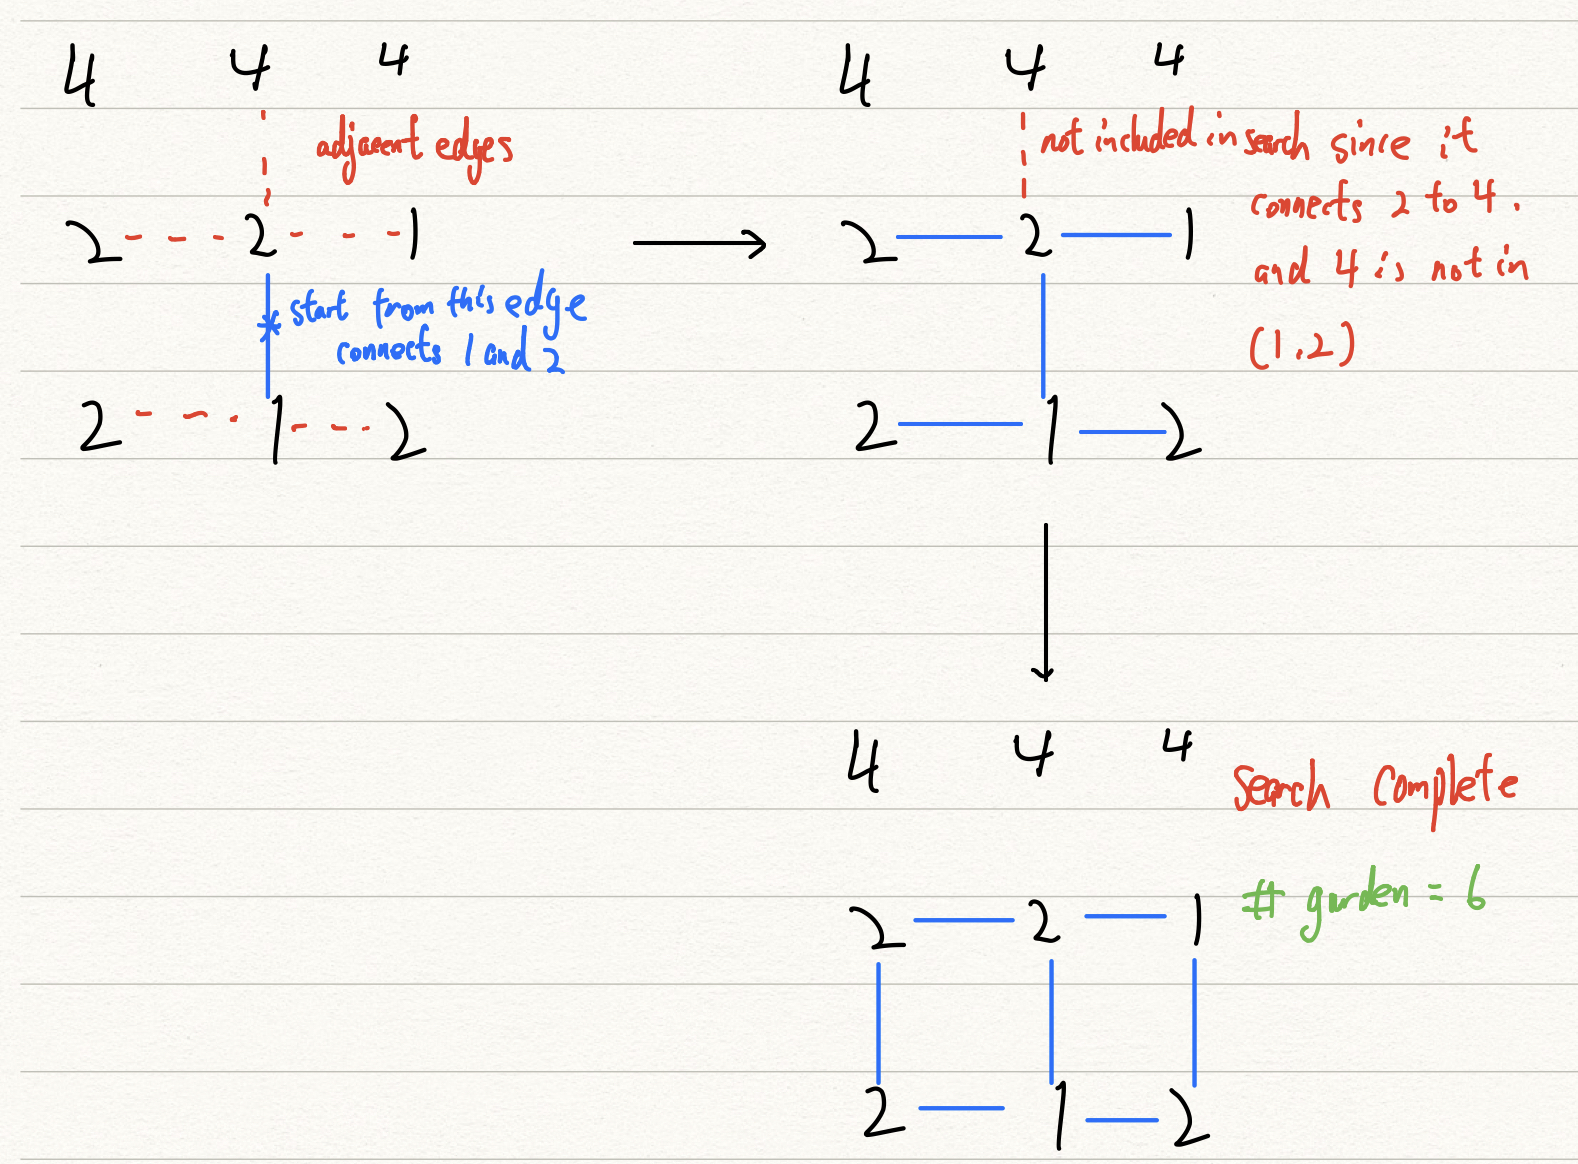
\includegraphics[width=0.9\columnwidth]{Q8(1).jpeg}
            \item
            Then, start another search from an unexplored edge that connects two gardens with different types of flowers, count the number of gardens included in this search and compare it with the current maximum number of garden that could be connected in a single search.
            \item
            Keep choosing an unexplored edge that connects two gardens with different types of flowers and do search from it until there's no unexplored edge that connects gardens with two different types of flowers. Return the maximum number of gardens that a single search could connect.\\
            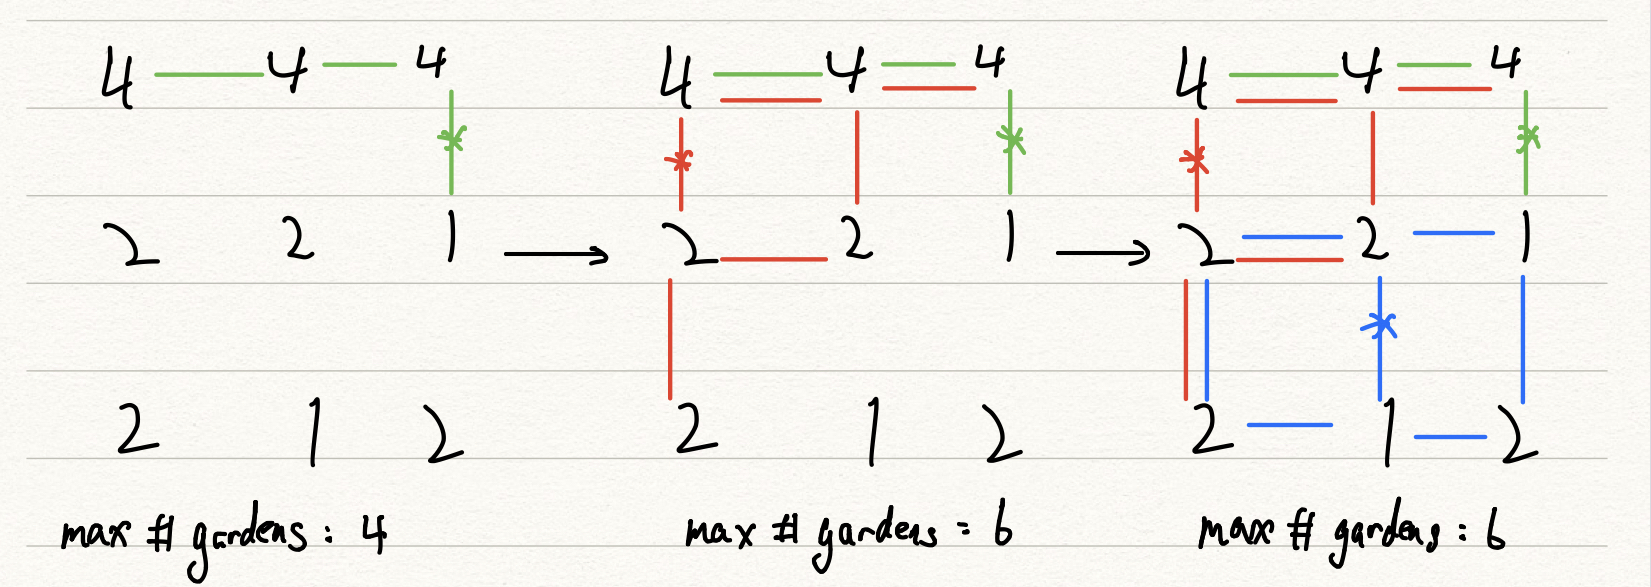
\includegraphics[width=0.9\columnwidth]{Q8(2).jpeg}
            This image shows how it works, note that edges with * is where every single search starts
            \item
            We could see that if an edge connects two gardens with same type of flowers, it could be visited at most $m-1$ times ($m$ is number of flower types), and if an edge connects two gardens with different types of flowers, it could be visited at most once. The number of edges connecting same type of flowers is $O(n^2)$, and $m$ is also $O(n^2)$. Nevertheless they are not independent with each other, thus the number of total edge visits in all searches within this field should be far less then $O(n^4)$. (Although I don't know how to mathematically calculate the complexity of this algorithm, I wrote a program to repeatedly randomly create a flower field, do those searches and count the number of total edge visits to get the maximum number of edge visits, and it is close to $O(n^2 \log n)$)
        \end{enumerate}
    \end{enumerate}
\end{answer}

\end{document}
\endinput
%%
%% End of file `ps4.ans.tex'.
